A miscellany of brief items in no particular order includes:

\begin{itemize}
\tightlist
\item
  Data downloads have been initiated for any presences I have on
  Twitter. It is questionable as to \emph{when} results will be
  available for download. Once those are complete those accounts will
  lay fallow.
\item
  I am scheduled to preach at
  \href{https://www.genevachurchofchrist.org/}{Geneva Church of Christ}
  on December 11th. My topic is yet to be determined.
\item
  Apparently my recent letters to the editor in \emph{The Star Beacon}
  inflamed quite a few Republicans locally to the point of expressing
  seemingly violent opinions that didn't happen to be ``true threat''
  levels of concern. That's kinda sad. It was very funny to see that
  they at least searched for me, found
  \href{https://erielookingproductions.info}{Erie Looking Productions},
  and then couldn't get the name right by calling it something stupid. I
  suspect I am being subjected to quite a bit of hideous name-calling on
  Facebook.
\item
  I still have to find a new episode to put up on
  \href{https://coyote.works/}{ELP Television}.
\item
  Yes, I am one of those folks expecting outbreaks of violence depending
  upon how the election turns out Tuesday. The MAGA people crave
  violence for no clear reason. I don't think they'll like it if they
  get what they're seeking, though.
\item
  I'm still considered locally to be a non-resident even though I am a
  homeowner, lost a race for city council, graduated from high school
  locally, and got an associate's degree at the local campus of Kent
  State University. Being neither Roman Catholic nor Lutheran let alone
  Pentacostal puts you well outside the ``good old boy network'' locally
  and leads to an interesting bit of social exclusion.
\item
  Work continues on trying to get WEFAX reception up in-house. The
  closest station would be NMF in Boston. Fortunately the western
  Atlantic charts still include Lake Erie in their scope.

  \begin{itemize}
  \tightlist
  \item
    It would be nice to get APT/LRPT reception up too but that would
    take quite a bit of work
  \item
    NAVTEX is seemingly contraindicated as the one station covering the
    Great Lakes has co-channel interference on 530 kHz from a station
    the CRTC isn't cracking down on sufficiently
  \item
    Getting licensed to make my own data blasts like that is difficult
    to comprehend in the present rules promulgated by the Commission
  \end{itemize}
\item
  I still need to look at finding space to set up an appropriate server
  running \href{https://citadel.org/}{Citadel} so as to have a BBS
  running.
\item
  I am still aware of the time shift and will handle it appropriately.
\end{itemize}

\begin{figure}
\centering
\pandocbounded{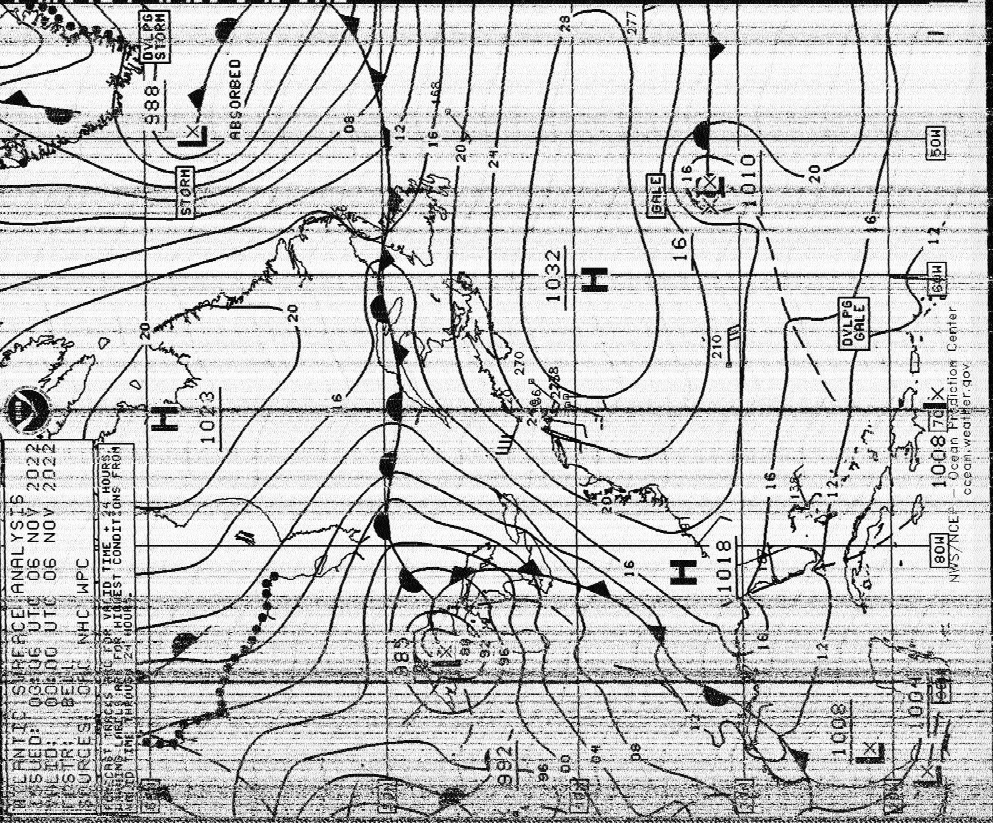
\includegraphics[keepaspectratio]{\%7B\%7Bsite.url\%7D\%7D/img/wefax2.jpg}}
\caption{A chart received using a WEFAX decoder plugin on a KiwiSDR
networked receiver in Ontario, Canada.}
\end{figure}
